\begin{frame}
\frametitle{MSAA: Demo}
\begin{figure}[ht]
    \centering
    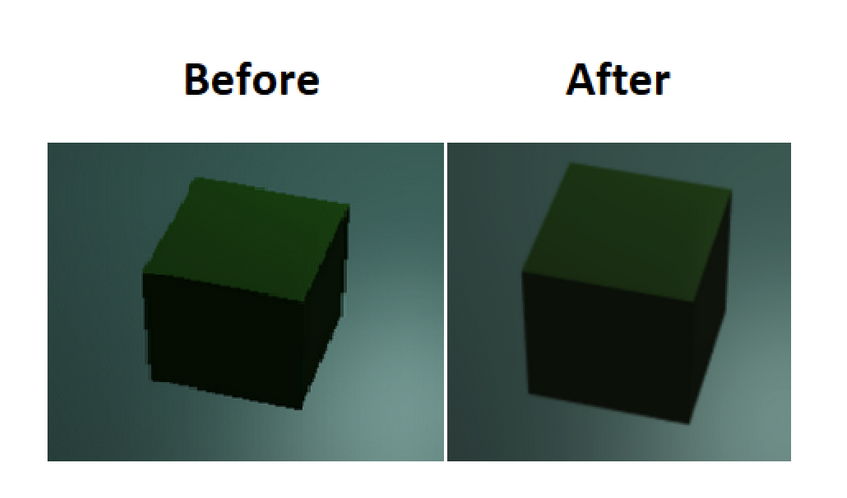
\includegraphics[scale=0.50]{images/SlidesMSAA/BeforeAfterMSAA.png}
\end{figure}
\end{frame}

\begin{frame}
\frametitle{MSAA: Un Campione Per Pixel}
\begin{figure}[ht]
    \centering
    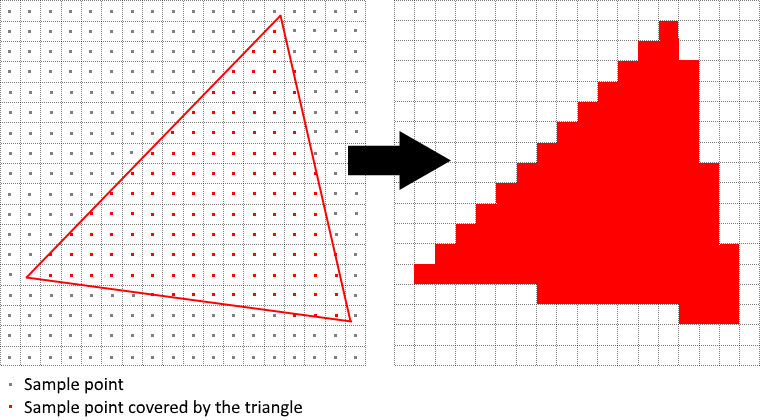
\includegraphics[scale=0.50]{images/SlidesMSAA/OneSamplePerPixel.png}
\end{figure}
\end{frame}

\begin{frame}
\frametitle{MSAA: Quattro Campioni Per Pixel}
\begin{figure}[ht]
    \centering
    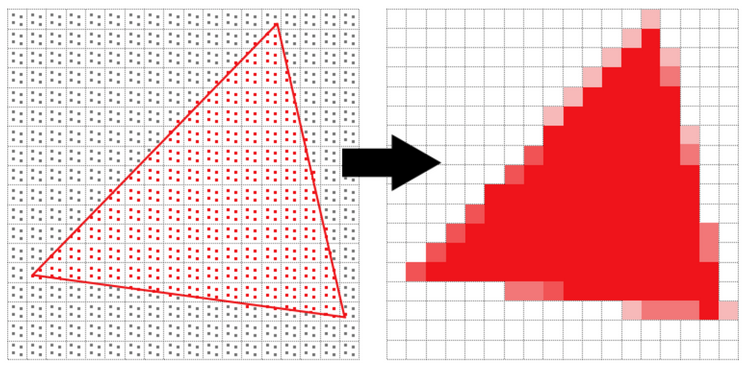
\includegraphics[scale=0.50]{images/SlidesMSAA/FourSamplesPerPixel.png}
\end{figure}
\end{frame}

\begin{frame}
\frametitle{MSAA}
\begin{itemize}
\item Le immagini che supportano il multisampling non sono presentabili
\item Tutte le immagini presentabili devono avere un solo campione per pixel
\item Creiamo una nuova immagine che abbia il numero di campioni per pixel che desideriamo
\item Useremo questa immagine come nuovo color attachment nel render pass
\item Usiamo l'immagine della swapchain come color resolve attachment
\item Non dobbiamo dimenticarci di abilitare il multisampling quando creiamo un pipeline state object
\end{itemize}
\end{frame}
